\section{Fases Abertas em Linhas de Transmissão - Religamento Monopolar}

Para o estudo de fases abertas em linhas de transmissão são necessários os conceitos básicos abaixo:

\begin{itemize}
    \item \textbf{Arco primário}: é o arco de potência formado pela cadeia de isoladores no caso de um curto-circuito fase-terra;
    \item \textbf{Arco secundário}: é a corrente que persiste devido ao acoplamento capacitivo e indutivo da fase defeituosa com as fases sãs após o seccionamento da fase defeituosa;
    \item \textbf{Polo preso}: condição do polo de um polo do disjuntor não operar em uma manobra de abertura;
    \item \textbf{Matriz admitância trifásica}: representa os acoplamentos indutivos e capacitivos da linha, outras linhas ou equivalentes do sistema e reatores;
\end{itemize}

\subsection{Representação da rede}
\subsubsection{Representação por matriz de admitâncias nodais}

Para a representação correta das redes é necessário estabelecer uma representação satisfatória da matriz de admitância dos reatores para poder incorporar à matriz de admitâncias da linha. Considerando reatores por fase de reatância $X$ ($Z = jX$ e $y = 1/x$), ter-se-á dois casos:


\begin{subquestion}
    \item Reatores monofásicos aterrados e possuem matriz admitância trifásica de:
    
\begin{equation} \label{slide:1}
    Y_r \, = \,\begin{bmatrix} y & 0 & 0 \\ 0 & y & 0 \\ 0 & 0 & y  \end{bmatrix}
\end{equation}

    \item Reatores monofásicos aterrados por meio de um reator de neutro ($X_n$) comum aos reatores e possuem matriz admitância trifásica para o reator de:
    
\begin{equation} \label{slide:2}
    Y \, = \,\begin{bmatrix} y & 0 & 0 & -y \\ 0 & y & 0 & -y \\ 0 & 0 & y & -y \\ -y & -y & -y & 3y+y_n  \end{bmatrix}
\end{equation}

Pela existência do reator de neutro, a reatância de sequência 0 não será mais igual às demais, resultando em: $X_1 = X_2 = X$ e $X_0 = 3X_n$. Aplicando a redução de Kron, eliminando uma equação da matriz anterior, permitindo representá-la como uma matriz 3x3.

\begin{equation} \label{slide:3}
    Y_r \, = \,\begin{bmatrix} y+k & k & k \\ k & y+k & k \\ k & k & y+k  \end{bmatrix}, \, \, \, com \, \,  k=-\frac{y^2}{3y+y_n}
\end{equation}
\end{subquestion}

Para a matriz de admitância da linha ($Y_{linha}$), são incluídos os efeitos da impedância série por meio da matriz de admitâncias $G_1$ e os efeitos das admitâncias capacitivas por $G_2$. Vale destacar que a matriz de admitâncias $Y_r$ pode ser inserida em qualquer terminal, representando a soma de $Y_r$ ao elemento desejado da diagonal principal de $Y_{linha}$. Assim, considerando a inserção no terminal 1 e 2:

\begin{equation} \label{slide:4}
    Y_a \, = \, Y_{linha} + \begin{bmatrix} Y_r & 0 \\ 0 & Y_r \end{bmatrix} \, = \, \begin{bmatrix} G_1+G_2 & -G_1 \\ -G_1 & G_1+G_2 \end{bmatrix} + \begin{bmatrix} Y_r & 0 \\ 0 & Y_r \end{bmatrix} \, = \, \begin{bmatrix} G_1+G_2+Y_r & -G_1 \\ -G_1 & G_1+G_2+Y_r \end{bmatrix}  
\end{equation}

Esse modelo permite uma representação completa da rede, podendo ser simplificada ao eliminar a matriz que representa impedâncias em série e resultam na queda de tensão.

\subsubsection{Representação por componentes simétricas}

A representação considera uma linha: trifásica, transposta, acoplamentos através da sequência positiva e zero, desprezando impedância série e acoplamento das fases pelas capacitâncias totais concentradas pontualmente.

Analisando o modelo com tensões de sequência positiva (tensões equilibradas) a tensão no neutro é nula. A capacitância resultante será $C_1$. No caso de tensões de sequência zero o modelo não possuirá diferença de potencial entre as fases uma vez que $V= [V_0;V_0;V_0]$ de forma que a corrente que circuita é a fase-terra na parte inferior do circuito. Por meio da capacitância mútua entre fases $C_m$, tem-se: $3C_m = C_1-C_0$, de forma que para ao transformar de estrela para triângulo de $C_1-C_0$ para $(C_1-C_0)/3$, resultando em uma capacitância entre fases de $C_0$.

Para reatores de compensação a análise é a mesma, resultando em um equivalente de $X_1$ para sequência positiva e $X_0$ para sequência zero.

Para um modelo mais completo de linha com reator, associa-se em paralelo ambos os modelos individuais para cada componente sequência.

Assim resulta na conclusão de que: quando não houver reator de neutro só é considerada a parte inferior do modelo pois $X_1 = X_0$. Desprezar a impedância do alimentador não causa problemas, pois esta é inferior às demais.

Assim, o modelo da linha com os capacitores e reatâncias será:

\begin{figure}[H]
\begin{center}
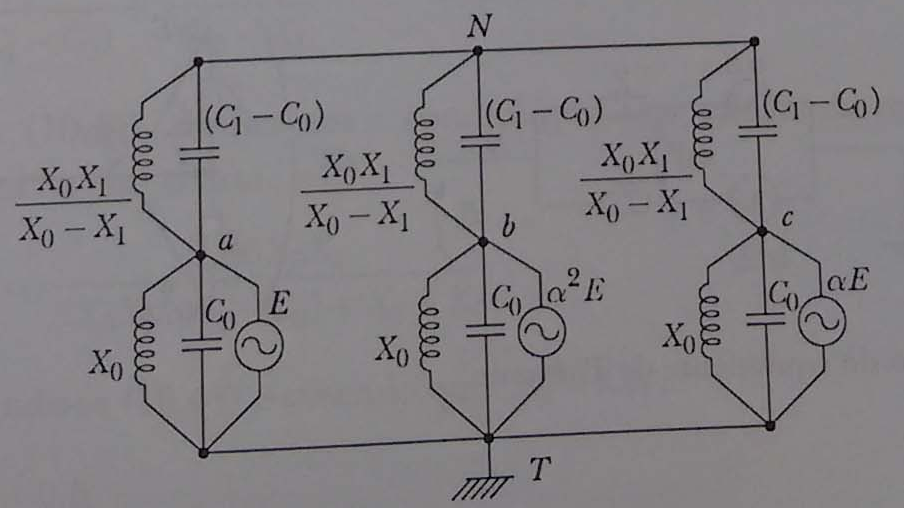
\includegraphics[width=8cm]{images/linha_reatores.png}
\caption{Modelo de linha com reatores acoplados. Fonte: Júnior, 2003.}
\label{fig:1} 
\end{center}
\end{figure}